\subsection{Sample Memory} \label{subsec:Sample_Memory} 
The Sample Control module will have to store \SIQ{320}{\kilo\bit} of sample data from the ADC before the MCU starts reading them, as mentioned in section \refq{subsubsec:CommunicationDatarate}. The Artix 7 FPGA development\cite{CMOD_A7_AT35T} board being used comes with \SIQ{4}{\mega\bit} of external asynchronous SRAM from ISSI\cite{ISSISRAM} that will be used to store the sampled data. The memory is organized as an array of 512K x 8 bit values, and because the ADC data are 16 bit values the Sample Control module should have hardware to store each sample in two distinct memory addresses in the external memory.

The IS61 SRAM has the functional block diagram shown on figure \refq{fig:7_2_5_IS61Block}.

\begin{figure}[H]
    \centering
    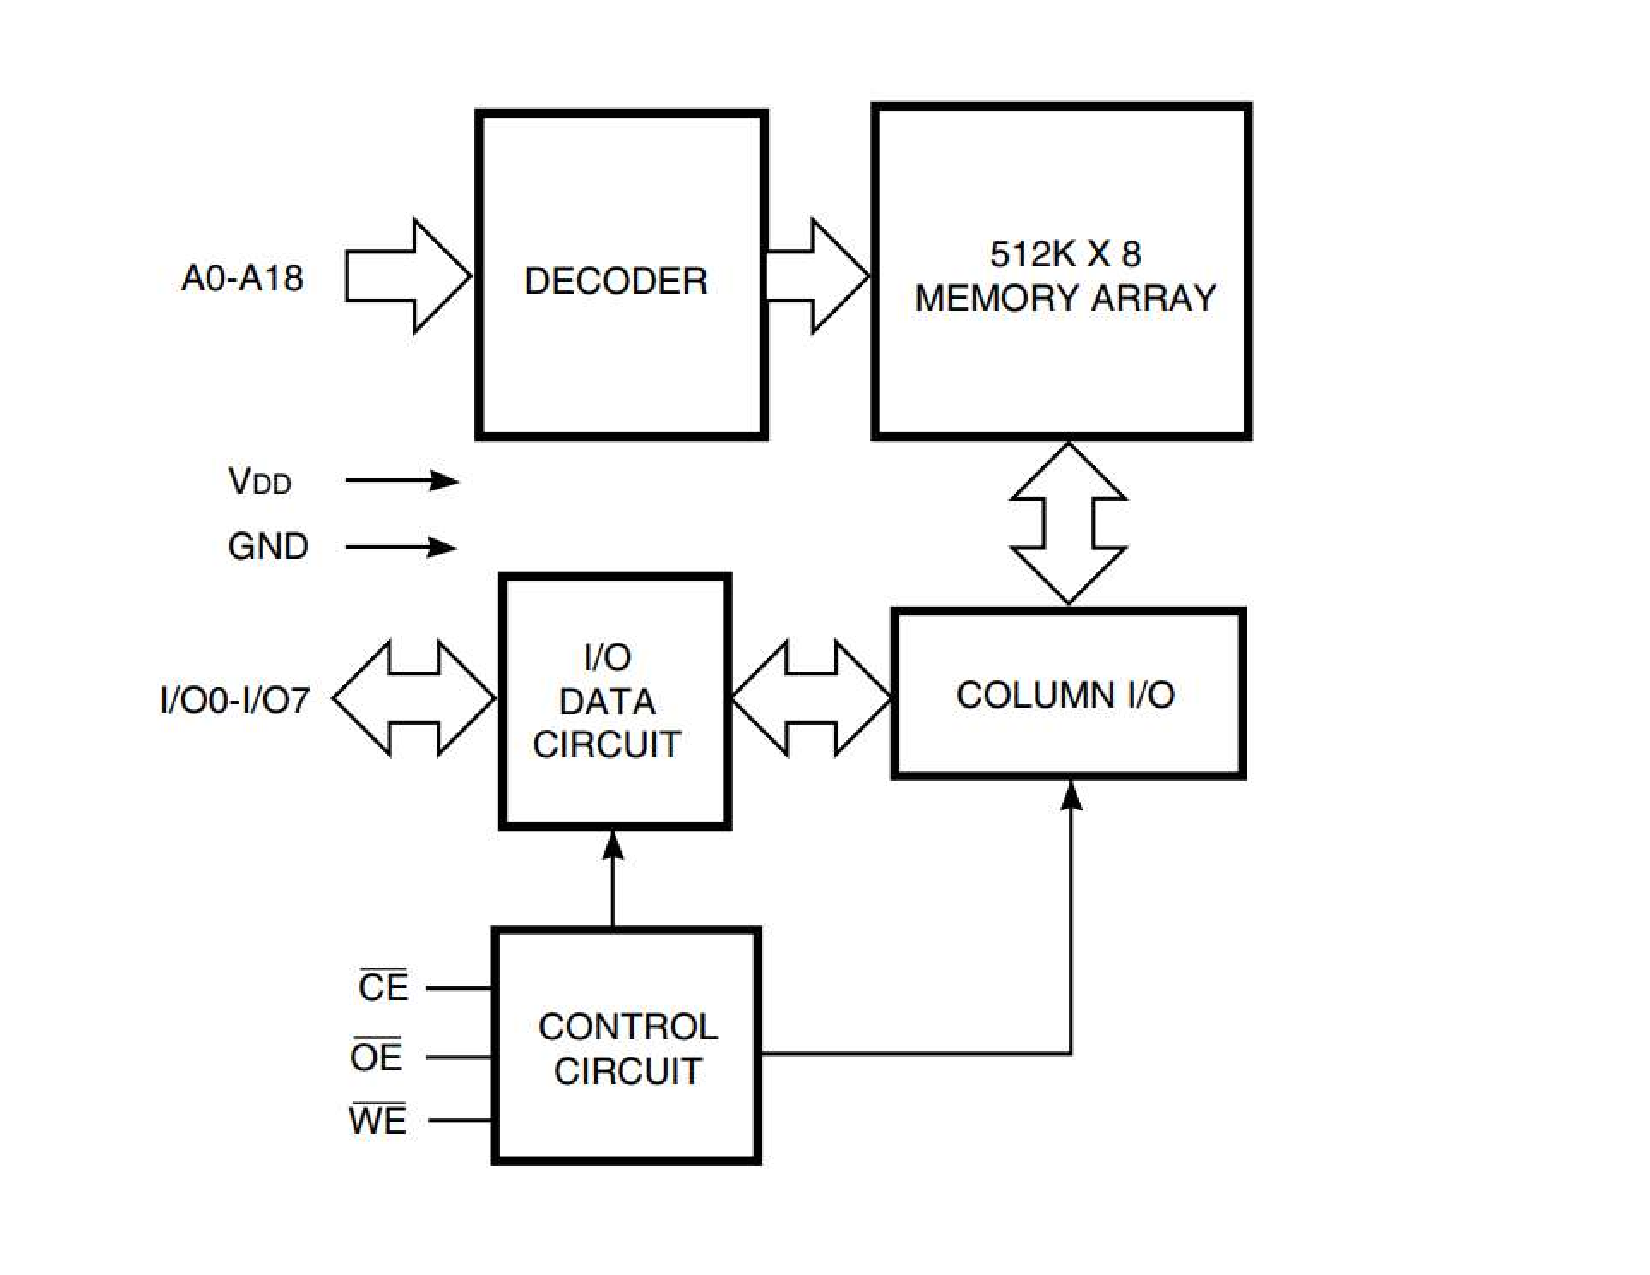
\includegraphics[clip, trim=0 0 0 0, width=0.65\textwidth]{Sections/7_SystemDesign/Figures/7_2_5_IS61_BLOCK_DIAGRAM.pdf}
    \caption{The functional block diagram for the IS61 SRAM\cite{ISSISRAM}. The SRAM uses a 19bit address bus, 8 bit bidirectional data bus along with 3 control signals.}
    \label{fig:7_2_5_IS61Block}
\end{figure}

The FPGA will have to control the address bus, data bus and control signals shown on figure \refq{fig:7_2_5_IS61Block} in order to write to, and read from, the IC. The control signals are Chip Enable (CE), Output Enable (OE) and Write Enable (WE) and they are all active-low signals. The CE input is used to put the the IC into a low-power standby mode, this is not used for this project, so CE is tied to logic '0' at all times. The OE signal controls the state of the output drivers on the chip and a '0' activates the outputs while a '1' sets them into a high impedance state. The WE input controls if a write or read is happening to/from the IC. Note how there is no clock signal, so the memory is asynchronous and any reads, or writes, happens when the WE signal changes state.

In order to write to RAM the FPGA should have hardware that follows the write cycle shown on figure \refq{fig:7_2_5_IS61_WRITE} from the IS61 datasheet.
\begin{figure}[H]
    \centering
    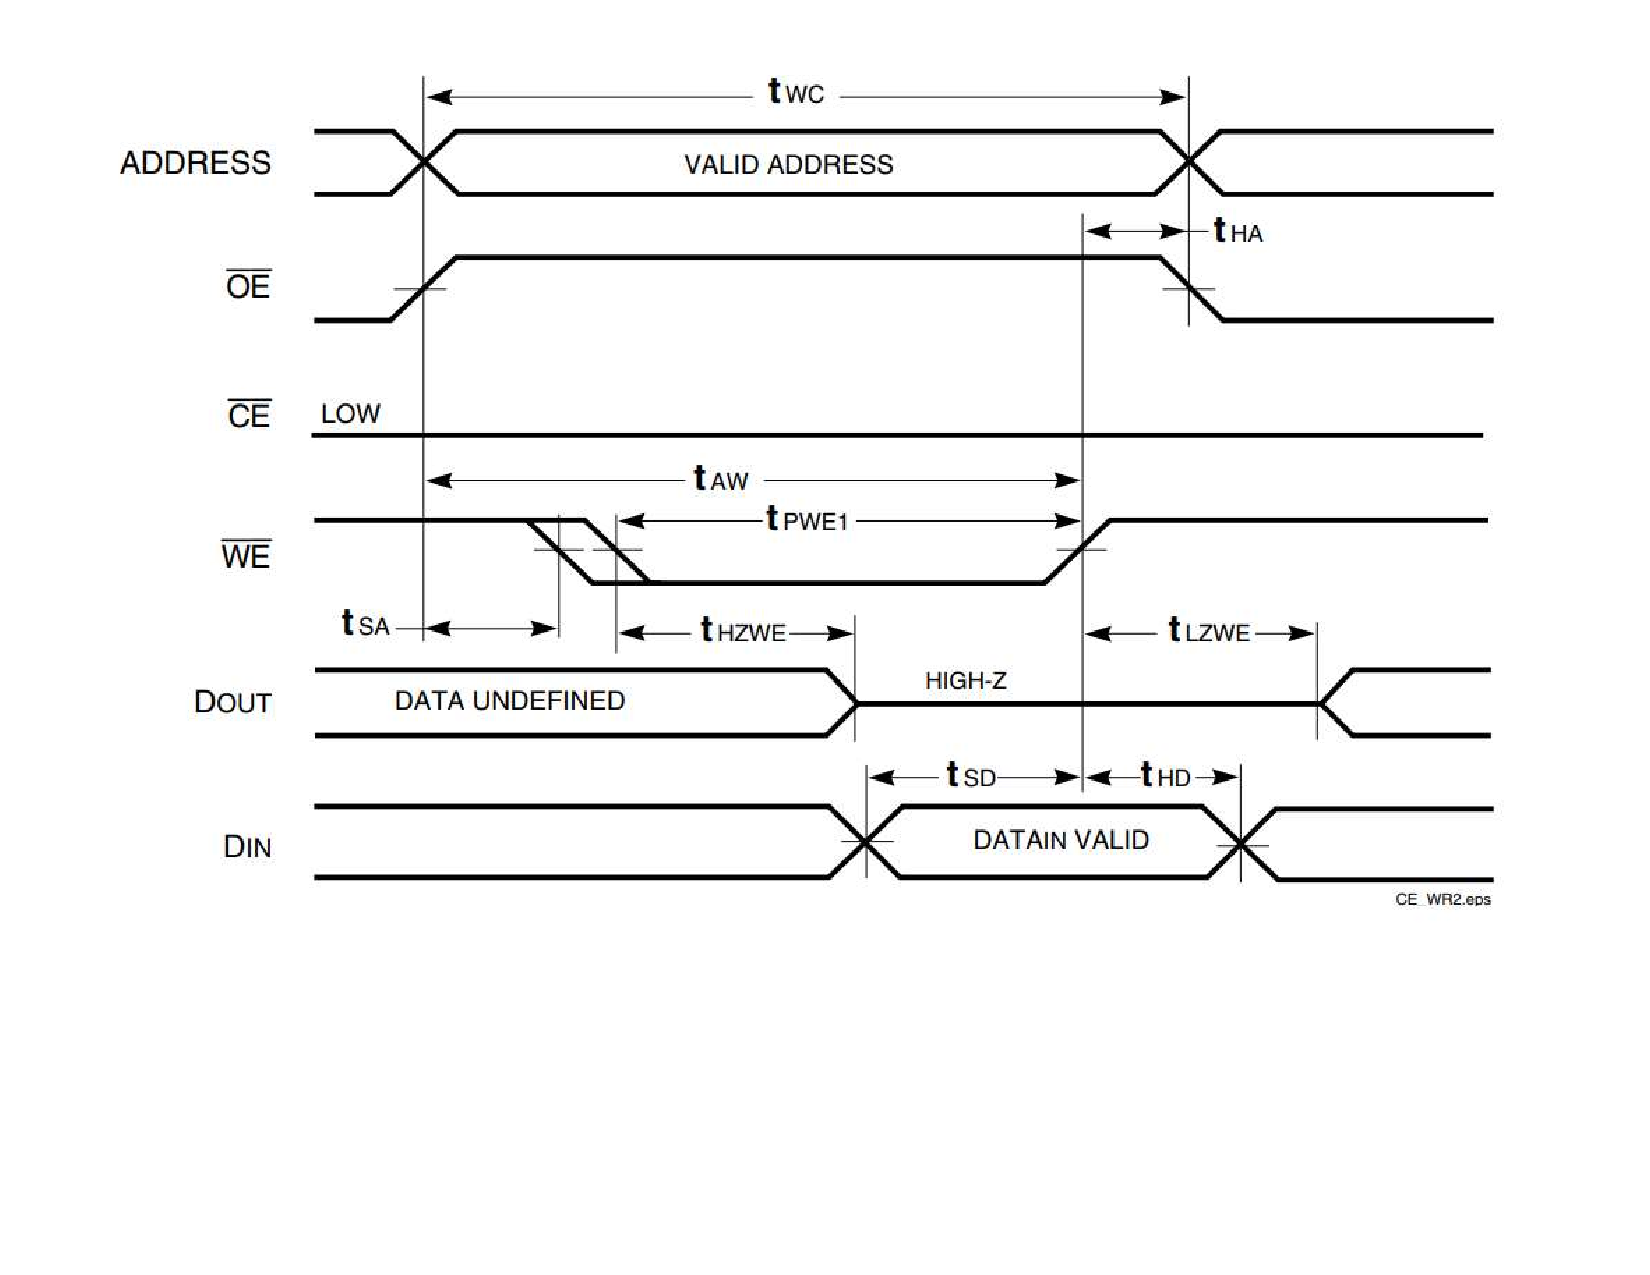
\includegraphics[clip, trim=0 150 0 0, width=0.8\textwidth]{Sections/7_SystemDesign/Figures/7_2_5_IS61_WriteCycle.pdf}
    \caption{A complete write cycle for the IS61 SRAM IC\cite{ISSISRAM}. In order to write to RAM the FPGA should go through the following sequence of events; Set Address to Address bus, Disable output drivers with OE = '1', assert Write Enable with WE = '0', set data to data bus and finish the sequence with WE = '1' to CLK the data byte into RAM.}
    \label{fig:7_2_5_IS61_WRITE}
\end{figure}

The write cycle begins by letting OE go from '0' to '1', the time from this event to WE going low is reffered to as $t_{SA}$ and should be a minimum of \SIQ{0}{\nano\second} according to the datasheet. Figure \ref{fig:7_2_5_IS61_WRITE} does however indicate that the address and OE should be configured before WE goes from '1' to '0'.

the time $t_{HZWE}$ is the time it takes for the output to be tristated after WE goes low, this takes \SIQ{2}{\nano\second} according to the datasheet. Finally there must go at least \SIQ{5}{\nano\second} from the output being tristated to WE going high again, "clocking" in the data on the data IO pins. These time constraints should be repsected for the chip to function properly. All timings are taken for the \SIQ{8}{\nano\second} write cycle chip, this depends on the supply voltage, the memory IC is supplied with \SIQ{3.3}{\volt}, resulting in a write cycle time of \SIQ{8}{\nano\second}, see the datasheet of the IC for more information on this.

The read and write cylces for controlling the memory IC are buid around a counter. If data is to be written or read from the external memory, a counter will increment by 1 at each rising edge of a \SIQ{200}{\mega\hertz} master clock. Depending on the variable of the counter the output of the process will take different states. The advantage of using a counter to advance this state machine is that the timeing constraints can be honored. The VHDL code for the counter can be seen in listing \ref{lst:7_2_5_FSM_COUNTER}. Here it can be seen that if a rising edge on the master clock occurs and the sequence is to run, the counter will increment by 1.

\lstinputlisting[language=C ,style = c,firstnumber=1, linerange=88-93, caption={VHDL code for the FSM counter incrementation.}, label={lst:7_2_5_FSM_COUNTER}]{Sections/7_SystemDesign/Code/EXT_MEM_RW20.vhd}

The write sequence shown on figure \refq{fig:7_2_5_IS61_WRITE} has been implemented in hardware as a state machine as shown in the code listing list \refq{lst:7_2_5_Write_SEQ}.

\lstinputlisting[language=C ,style = c,firstnumber=1, linerange=105-121, caption={VHDL code for the write sequence process.}, label={lst:7_2_5_Write_SEQ}]{Sections/7_SystemDesign/Code/EXT_MEM_RW20.vhd}

When the "v\_Count" is less or equal to 1, this it will be at the first rising edge of the master clock, the address will be set and output enable will be set to a logical '1'. The output data is also set at this point, however the output data is not presented to the IC yet, as a control signal will enable the output buffer at a later state. 

The next rising edge of the master clock will have "v\_Count" take the value 2, and output enable is set to a logical '0'. Here a time of \SIQ{5}{\nano\second} has passend since the last changes due to the period of the master clock being \SIQ{5}{\nano\second}. The time constraint from write enable going low to the data on the datalines being valid is requied to be \SIQ{5}{\nano\second}, to ensure this is honored, two clocks are required to arise before the output buffer is changed from being tristated to being enabled, hence the elsif "v\_Count = 4" statement. Hereafter write enable is set to a logical '1', clokcing in the data. on the next clock the output is once again tristated and the sequence is completed. 

This sequence requires 7 master clocks to be completed and thus it takes \SIQ{35}{\nano\second} to write a single byte to the external memory. This allows for a data-rate of \SIQ{228}{\mega\bit/\second}.

The read cycle for the IS61 SRAM follows a similar procedure as shown on the read cycle timing diagram on figure \refq{fig:7_2_5_IS61_READ}.
\begin{figure}[H]
    \centering
    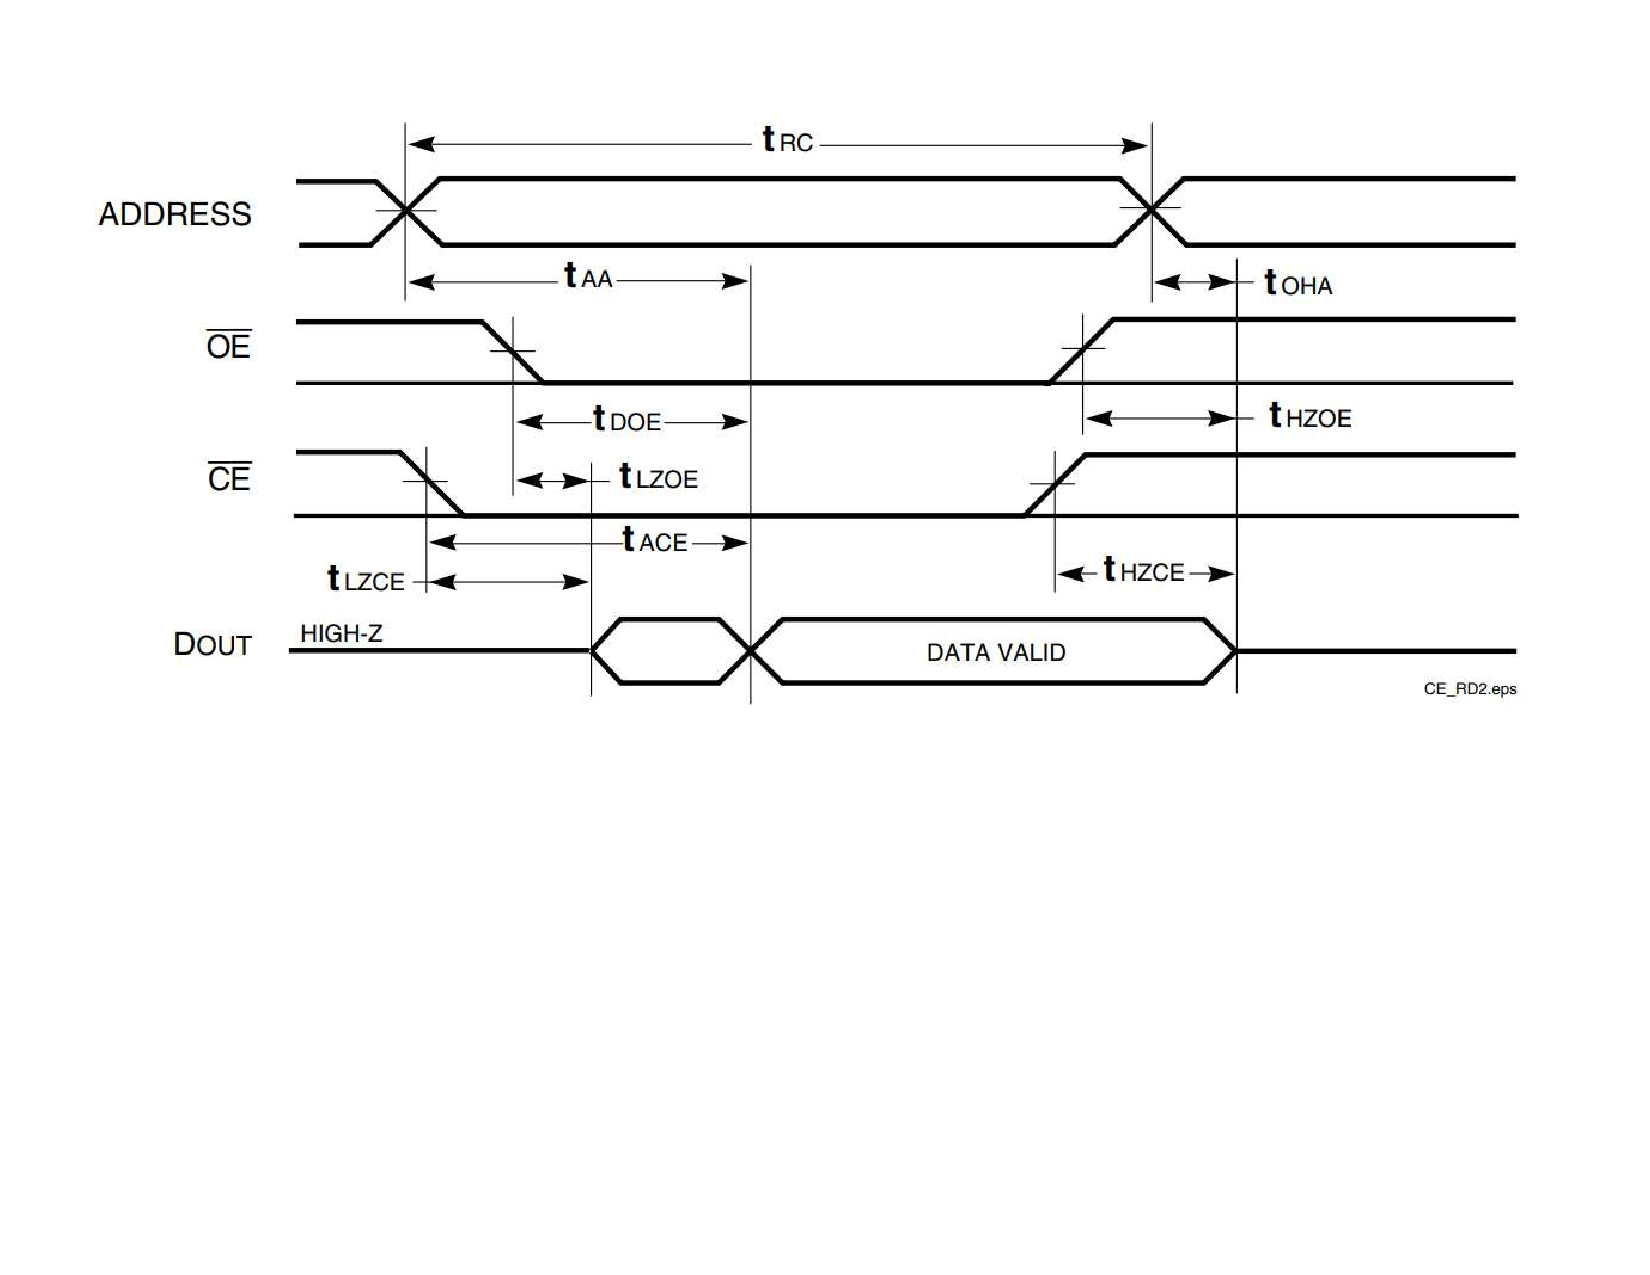
\includegraphics[clip, trim=0 250 0 0, width=0.8\textwidth]{Sections/7_SystemDesign/Figures/7_2_5_IS61_ReadCycle.pdf}
    \caption{A complete read cycle for the IS61 SRAM IC\cite{ISSISRAM}. An address must be set to the address bus, when an address is set the output drivers are enable with OE = '0'. Data is available on the data bus when OE transitions back to OE = '1'. CE is not being controlled in this projects application and is tied to logic '0'.}
    \label{fig:7_2_5_IS61_READ}
\end{figure}

Note how on figure \refq{fig:7_2_5_IS61_READ} the WE signal is not displayed, but WE should be held high for a read cycle in order to work properly. The CE signal is, also, not being controlled in this project and is still tied to '0'. The read cycle is also being controlled by a state machine and the code listing for this can be seen on listing \refq{lst:7_2_5_READ_SEQ}. The time $t_{AA}$ is the time the SRAM uses to fetch the data stored on whatever address is on the address line. With a \SIQ{3.3}{\volt} supply, this time is \SIQ{8}{\nano\second}, this constraint must be respected if proper functionality is to be expected.


\lstinputlisting[language=C ,style = c,firstnumber=1, linerange=94-105, caption={VHDL code for the read sequence state machine}, label={lst:7_2_5_READ_SEQ}]{Sections/7_SystemDesign/Code/EXT_MEM_RW20.vhd} 

The FSM shown in listing \refq{lst:7_2_5_READ_SEQ}  shows that when the sequence is initialized, output enable is set to '0', and a delay of two clocks is then present before the output buffer is tristated, note that the output buffer should already be tristated, but it is forced here as a means of good practice. On the third clock the address that is to be read from is set on the address line. When 6 clocks have occurred, the data on the datalines is latched in on the output data line of the module. The sequence is also set to be complete. This sequence takes 7 clocks to complete aswell or \SIQ{35}{\nano\second}. 

The whole sequence is initialized by the VHDL code shown in listing \ref{lst:7_2_5_start_SEQ}. If "w\_CMPLT" is set to "CMPLT or "i\_RESET" is set to '1', the process will set "w\_RUN" to '0', this will stop the process that Reads/Writes data to the external memory IC. If a rising edge on "i\_EN" arises "w\_RUN" will be set to RUN and the process to Read or Write to the IC will be initialized. Notice also the output "o\_ACTIVE" is "w\_RUN or w\_CMPLT", this results in "o\_ACTIVE" being '1'' for as long as the process is running. Once the process is done reading from or wrtting to the IC, "o\_ACTIVE" will be low. This can be used by other modules to see when the process is complete and new data can be send to this module.

\lstinputlisting[language=C ,style = c,firstnumber=1, linerange=77-86, caption={VHDL code for the read sequence initialization.}, label={lst:7_2_5_start_SEQ}]{Sections/7_SystemDesign/Code/EXT_MEM_RW20.vhd} 

The complete VHDL code for the Sample Memory can be seen in appendix \ref{App:EXT_MEM_RW_CODE}.

\subsubsection{IO Port}
The IO port used is one that can be configured both as an input and an output. A generic component from Xilinx has been used in exaclty the same way as for the FPGA and MCU communication. For more detail on this IO port see section \ref{subsec:Communication}. The signal used to enable or tristate the 8 bit IO datalines to the memory IC is the signal called "o\_IO\_BUF\_CTRL". When this signal is a logical '0' the output buffer is enabled, driving the output.